\newpage
\section{Anhang}

\subsection{Tabellen}


\begin{table}[ht]
    \centering
    \tiny
    \caption{Maxima der Messung für die Spin-Gitter Relaxationszeit.}
    \label{tab:T2}
    \begin{tabular}{S [table-format=1.6] S [table-format=1.6] |S [table-format=1.6] S [table-format=1.6]}
     \toprule
     {$\tau\mathbin{\scalebox{1.5} / } \si{\second}$} & $\text{Spannungsamplitude} \mathbin{\scalebox{1.5} / } \si{\volt}$ & {$\tau\mathbin{\scalebox{1.5} / } \si{\second}$} & $\text{Spannungsamplitude} \mathbin{\scalebox{1.5} / } \si{\volt}$\\
     \midrule
     0.001   & 0.883166   &   1.12075 & 0.482412 \\
     0.02075 & 0.81407    &   1.12275 & 0.462312 \\
     0.02275 & 0.844221   &   1.14275 & 0.472362 \\
     0.04275 & 0.854271   &   1.14475 & 0.462312 \\
     0.045   & 0.822864   &   1.16475 & 0.452261 \\
     0.06475 & 0.80402    &   1.167   & 0.440955 \\
     0.06675 & 0.78392    &   1.18675 & 0.452261 \\
     0.08675 & 0.844221   &   1.18875 & 0.442211 \\
     0.08875 & 0.854271   &   1.20875 & 0.462312 \\
     0.10875 & 0.79397    &   1.21075 & 0.472362 \\
     0.111   & 0.822864   &   1.23075 & 0.432161 \\
     0.13075 & 0.773869   &   1.23275 & 0.42211  \\
     0.13275 & 0.78392    &   1.25275 & 0.452261 \\
     0.15275 & 0.773869   &   1.255   & 0.440955 \\
     0.15475 & 0.81407    &   1.27475 & 0.41206  \\
     0.17475 & 0.743719   &   1.27675 & 0.452261 \\
     0.17675 & 0.80402    &   1.29675 & 0.432161 \\
     0.19675 & 0.773869   &   1.29875 & 0.432161 \\
     0.19875 & 0.79397    &   1.31875 & 0.39196  \\
     0.21875 & 0.733668   &   1.321   & 0.420854 \\
     0.221   & 0.762563   &   1.34075 & 0.41206  \\
     0.24075 & 0.723618   &   1.34275 & 0.42211  \\
     0.24275 & 0.733668   &   1.36275 & 0.42211  \\
     0.26275 & 0.733668   &   1.36475 & 0.39196  \\
     0.265   & 0.742462   &   1.38475 & 0.39196  \\
     0.28475 & 0.703518   &   1.38675 & 0.40201  \\
     0.28675 & 0.733668   &   1.40675 & 0.41206  \\
     0.30675 & 0.683417   &   1.40875 & 0.40201  \\
     0.30875 & 0.763819   &   1.42875 & 0.39196  \\
     0.32875 & 0.713568   &   1.43075 & 0.38191  \\
     0.33075 & 0.743719   &   1.45075 & 0.39196  \\
     0.35075 & 0.713568   &   1.45275 & 0.40201  \\
     0.35275 & 0.733668   &   1.47275 & 0.38191  \\
     0.37275 & 0.683417   &   1.47475 & 0.40201  \\
     0.37475 & 0.733668   &   1.49475 & 0.390703 \\
     0.39475 & 0.673367   &   1.49675 & 0.371859 \\
     0.39675 & 0.703518   &   1.51675 & 0.371859 \\
     0.41675 & 0.673367   &   1.519   & 0.380653 \\
     0.41875 & 0.713568   &   1.53875 & 0.371859 \\
     0.43875 & 0.653266   &   1.54075 & 0.361809 \\
     0.44075 & 0.683417   &   1.56075 & 0.361809 \\
     0.46075 & 0.653266   &   1.56275 & 0.361809 \\
     0.463   & 0.621859   &   1.58275 & 0.351759 \\
     0.48275 & 0.653266   &   1.585   & 0.380653 \\
     0.485   & 0.66206    &   1.60475 & 0.361809 \\
     0.50475 & 0.603015   &   1.60675 & 0.361809 \\
     0.507   & 0.66206    &   1.62675 & 0.351759 \\
     0.52675 & 0.643216   &   1.62875 & 0.341709 \\
     0.529   & 0.66206    &   1.64875 & 0.331658 \\
     0.54875 & 0.643216   &   1.65075 & 0.351759 \\
     0.55075 & 0.643216   &   1.67075 & 0.341709 \\
     0.57075 & 0.633166   &   1.67275 & 0.351759 \\
     0.57275 & 0.592965   &   1.69275 & 0.341709 \\
     0.59275 & 0.613065   &   1.69475 & 0.361809 \\
     0.59475 & 0.653266   &   1.71475 & 0.341709 \\
     0.61475 & 0.613065   &   1.71675 & 0.341709 \\
     0.61675 & 0.623116   &   1.737   & 0.320352 \\
     0.63675 & 0.603015   &   1.73875 & 0.331658 \\
     0.63875 & 0.592965   &   1.75875 & 0.331658 \\
     0.65875 & 0.603015   &   1.76075 & 0.311558 \\
     0.66075 & 0.623116   &   1.78075 & 0.301507 \\
     0.681   & 0.601759   &   1.78275 & 0.311558 \\
     0.683   & 0.601759   &   1.803   & 0.300251 \\
     0.70275 & 0.552764   &   1.805   & 0.340452 \\
     0.705   & 0.601759   &   1.825   & 0.300251 \\
     0.72475 & 0.562814   &   1.82675 & 0.301507 \\
     0.727   & 0.601759   &   1.847   & 0.320352 \\
     0.74675 & 0.582915   &   1.849   & 0.300251 \\
     0.74875 & 0.592965   &   1.86875 & 0.301507 \\
     0.76875 & 0.552764   &   1.87075 & 0.321608 \\
     0.77075 & 0.552764   &   1.89075 & 0.301507 \\
     0.79075 & 0.572864   &   1.89275 & 0.311558 \\
     0.79275 & 0.572864   &   1.91275 & 0.301507 \\
     0.81275 & 0.572864   &   1.91475 & 0.311558 \\
     0.81475 & 0.562814   &   1.93475 & 0.291457 \\
     0.83475 & 0.532663   &   1.93675 & 0.291457 \\
     0.83675 & 0.552764   &   1.95675 & 0.290201 \\
     0.85675 & 0.542714   &   1.95875 & 0.281407 \\
     0.85875 & 0.552764   &   1.97875 & 0.301507 \\
     0.87875 & 0.551508   &   1.981   & 0.300251 \\
     0.88075 & 0.522613   &   2.00075 & 0.301507 \\
     0.90075 & 0.502513   &   2.003   & 0.300251 \\
     0.903   & 0.521357   &   2.02275 & 0.281407 \\
     0.923   & 0.501256   &   2.02475 & 0.291457 \\
     0.92475 & 0.522613   &   2.04475 & 0.281407 \\
     0.94475 & 0.502513   &   2.04675 & 0.261306 \\
     0.94675 & 0.522613   &   2.06675 & 0.251256 \\
     0.96675 & 0.512563   &   2.06875 & 0.281407 \\
     0.96875 & 0.512563   &   2.08875 & 0.271357 \\
     0.98875 & 0.492462   &   2.09075 & 0.281407 \\
     0.99075 & 0.512563   &   2.11075 & 0.261306 \\
     1.01075 & 0.472362   &   2.113   & 0.280151 \\
     1.013   & 0.521357   &   2.13275 & 0.271357 \\
     1.03275 & 0.492462   &   2.13475 & 0.261306 \\
     1.035   & 0.501256   &   2.15475 & 0.261306 \\
     1.05475 & 0.482412   &   2.15675 & 0.281407 \\
     1.05675 & 0.502513   &   2.17675 & 0.261306 \\
     1.07675 & 0.482412   &   2.179   & 0.280151 \\
     1.07875 & 0.492462   &   2.19875 & 0.261306 \\
     1.09875 & 0.442211   &   2.20075 & 0.271357 \\
     1.101   & 0.501256  & &\\
    \end{tabular}
  \end{table} 

%\begin{figure}[h]
%    \centering
%    \includegraphics[width=0.7\textwidth]{latex/images/messwerte.jpeg}
%    \caption{Die Messwerte der Interferenzmaximaanzahl}
%    \label{img:mess1}
%\end{figure}
%  
%\begin{figure}[h]
%    \centering
%    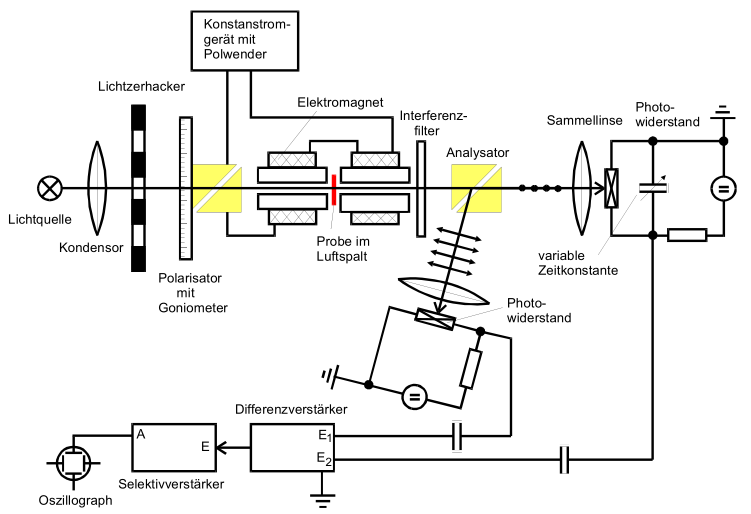
\includegraphics[width=0.7\textwidth]{latex/images/Aufbau.jpeg}
%    \caption{Der Versuchsaufbau des Michelson-Interferometers}
%\end{figure}